\documentclass[11pt]{article}
\usepackage[sort]{natbib}
\usepackage{bm,amsmath,bbm,amsfonts,nicefrac,latexsym,amsmath,amsfonts,amsbsy,amscd,amsxtra,amsgen,amsopn,bbm,amsthm,amssymb,graphicx, color, caption, subcaption}
\usepackage{fancyhdr, pbox}
\usepackage[margin=0.7in]{geometry}
\usepackage[english]{babel}
\usepackage[section]{placeins}
\usepackage{wrapfig}
\usepackage{lscape}
\usepackage{rotating}
\usepackage{epstopdf}
\bibliographystyle{plainnat}

\title{New Figure Ideas CVT}
\author{Ewan Pinnington}

\newtheorem{theorem}{Theorem}[section]
\newtheorem*{defn}{Definition}


\begin{document}

\maketitle

\begin{figure}
    \centering
    \begin{subfigure}[b]{0.49\textwidth}
        \includegraphics[width=\textwidth]{cost.eps}
        \caption{$|1-f(\alpha)|$}
        \label{fig:4dvardiagBR}
    \end{subfigure}
    \begin{subfigure}[b]{0.49\textwidth}
        \includegraphics[width=\textwidth]{costone.eps}
        \caption{$f(\alpha)$}
        \label{fig:4dvaredcBR}
    \end{subfigure}
    \begin{subfigure}[b]{0.49\textwidth}
        \includegraphics[width=\textwidth]{cost_cvt.eps}
        \caption{$|1-f(\alpha)|$ CVT}
        \label{fig:4dvarBcorR}
    \end{subfigure}
    \begin{subfigure}[b]{0.49\textwidth}
        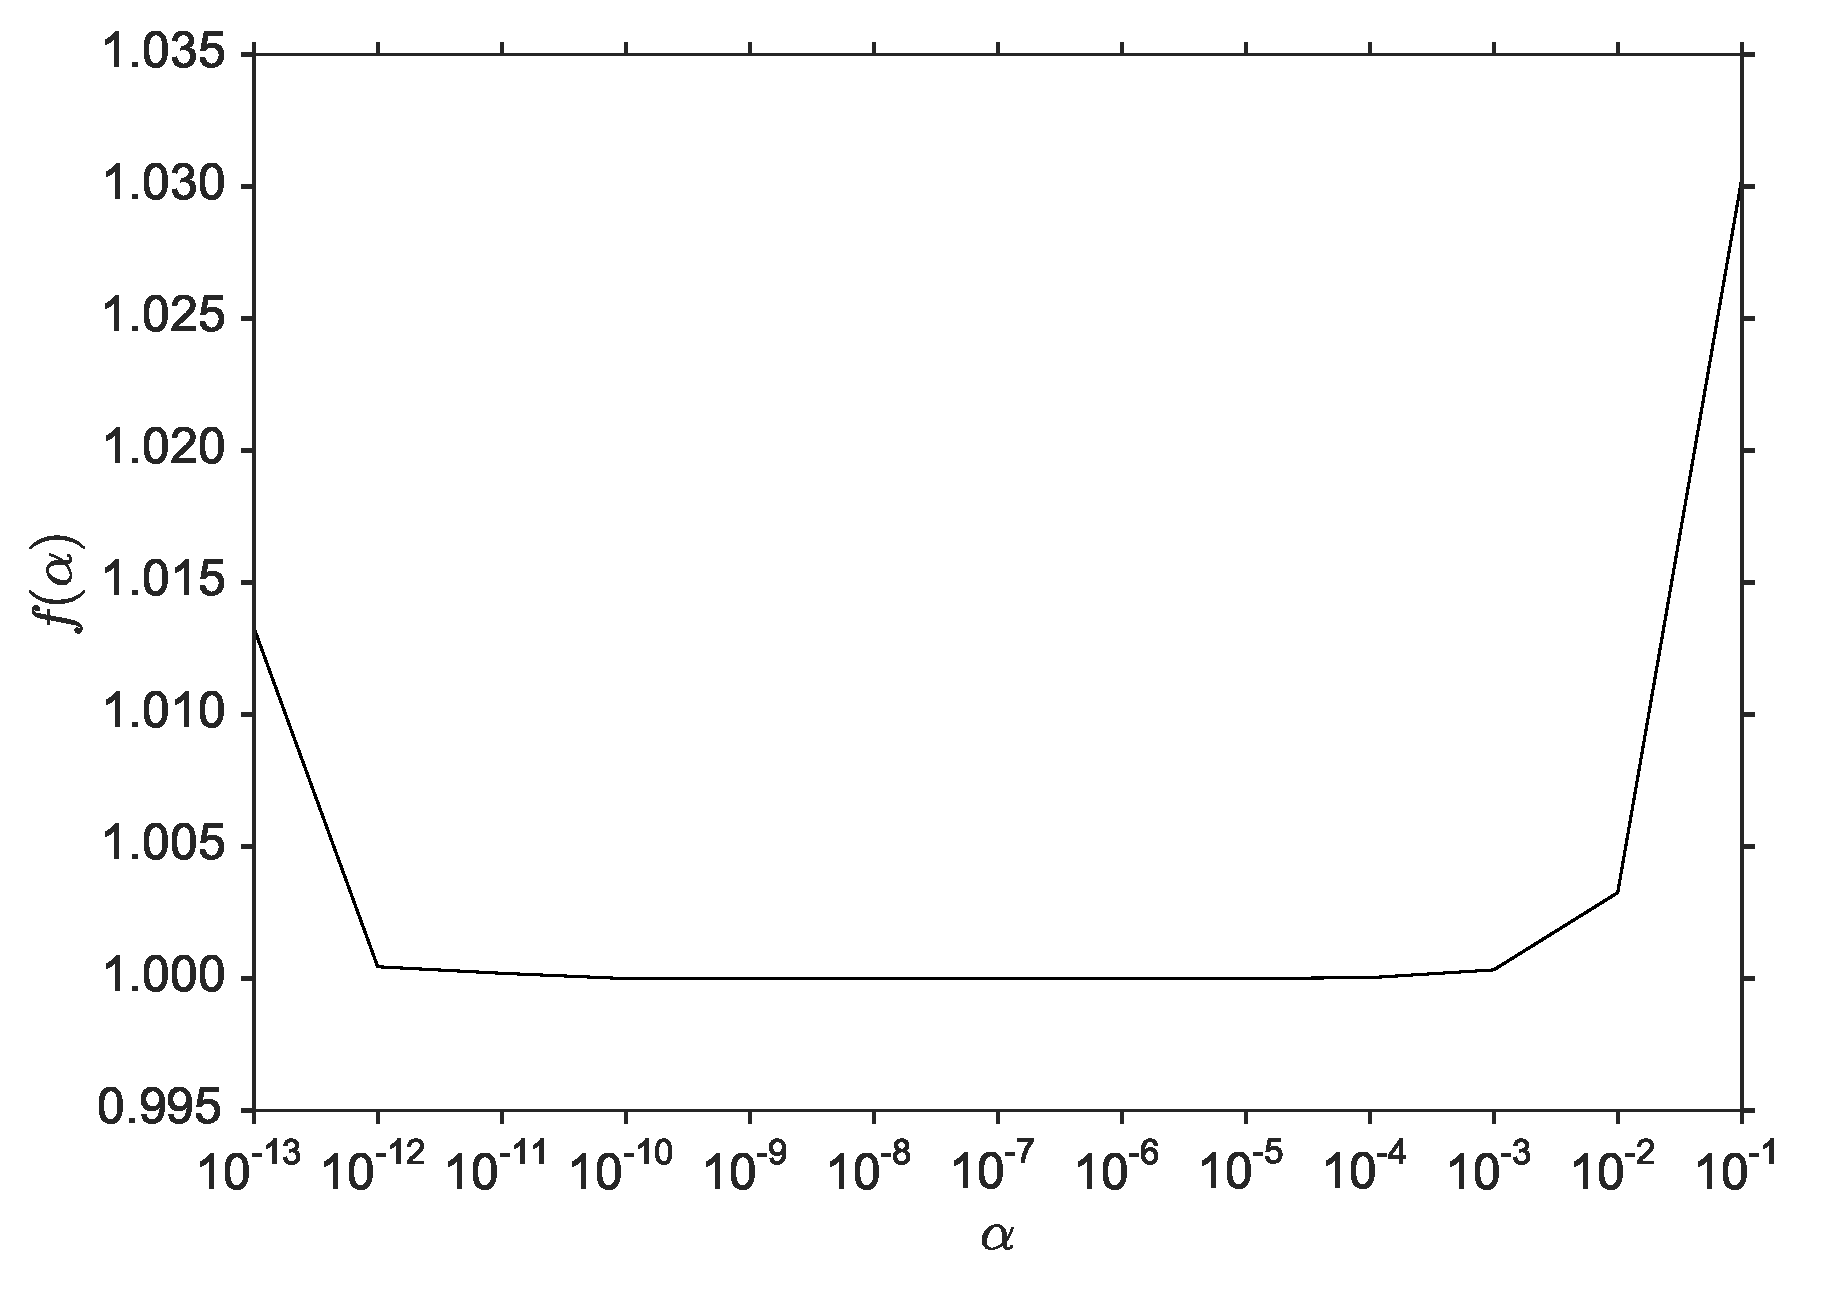
\includegraphics[width=\textwidth]{costone_cvt.eps}
        \caption{$f(\alpha)$ CVT}
        \label{fig:4dvaredcBcorR}
    \end{subfigure}
    \caption{Tests of gradient of the cost function.}\label{fig:4dvar}
\end{figure}

\begin{figure}
    \centering
    \begin{subfigure}[b]{0.49\textwidth}
        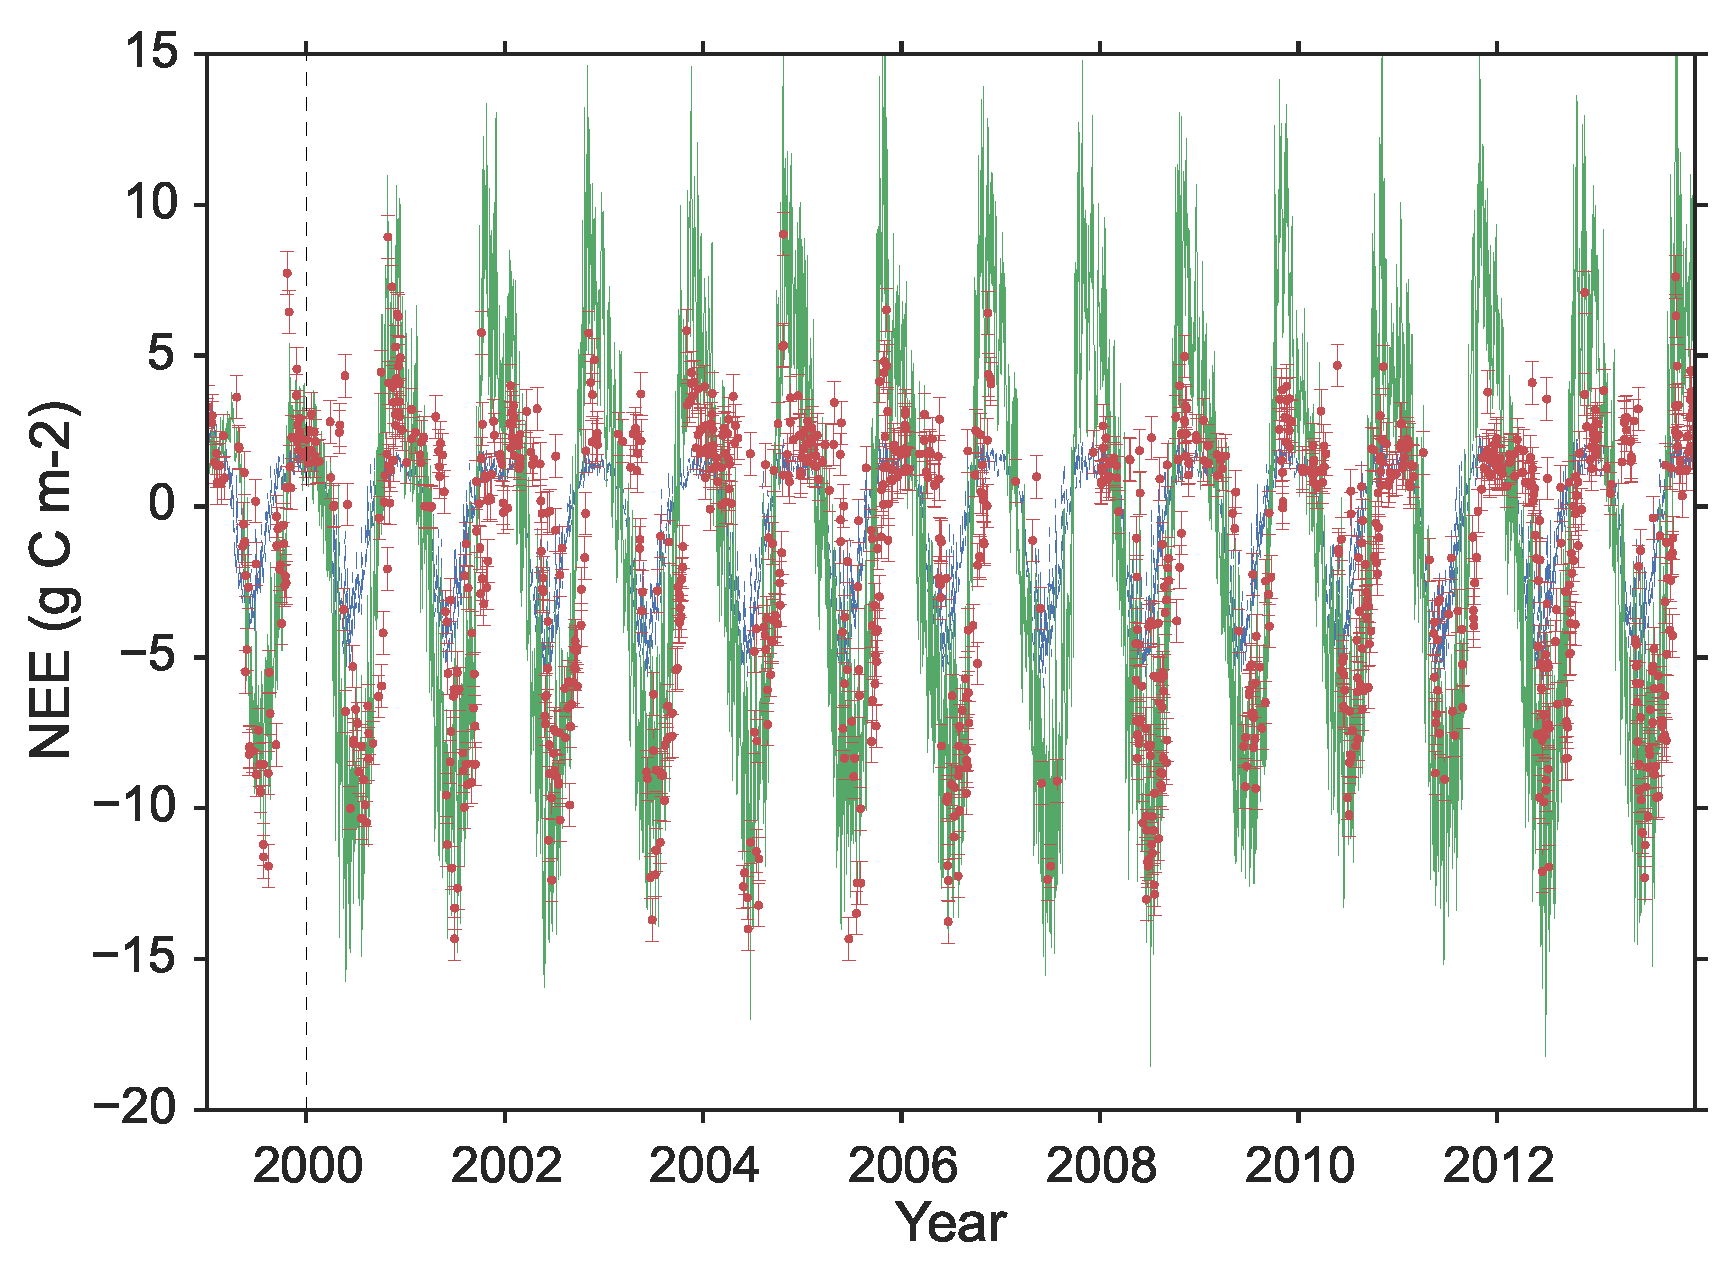
\includegraphics[width=\textwidth]{A4dvarcvt.eps}
        \caption{Experiment A}
        \label{fig:4dvardiagBR}
    \end{subfigure}
    \begin{subfigure}[b]{0.49\textwidth}
        \includegraphics[width=\textwidth]{B4dvarcvt.eps}
        \caption{Experiment B}
        \label{fig:4dvaredcBR}
    \end{subfigure}
    \begin{subfigure}[b]{0.49\textwidth}
        \includegraphics[width=\textwidth]{C4dvarcvt.eps}
        \caption{Experiment C}
        \label{fig:4dvarBcorR}
    \end{subfigure}
    \begin{subfigure}[b]{0.49\textwidth}
        \includegraphics[width=\textwidth]{D4dvarcvt.eps}
        \caption{Experiment D}
        \label{fig:4dvaredcBcorR}
    \end{subfigure}
    \caption{CVT: One year assimilation and fourteen year forecast of Alice Holt NEE with DALEC2, blue dotted line: background model trajectory, green line: analysis and forecast after assimilation, red dots: observations from Alice Holt flux site with error bars.}\label{fig:4dvar}
\end{figure}

\begin{figure}
    \centering
    \begin{subfigure}[b]{0.49\textwidth}
        \includegraphics[width=\textwidth]{Abroke4dvarcvt.eps}
        \caption{Experiment A}
        \label{fig:4dvardiagBR}
    \end{subfigure}
    \begin{subfigure}[b]{0.49\textwidth}
        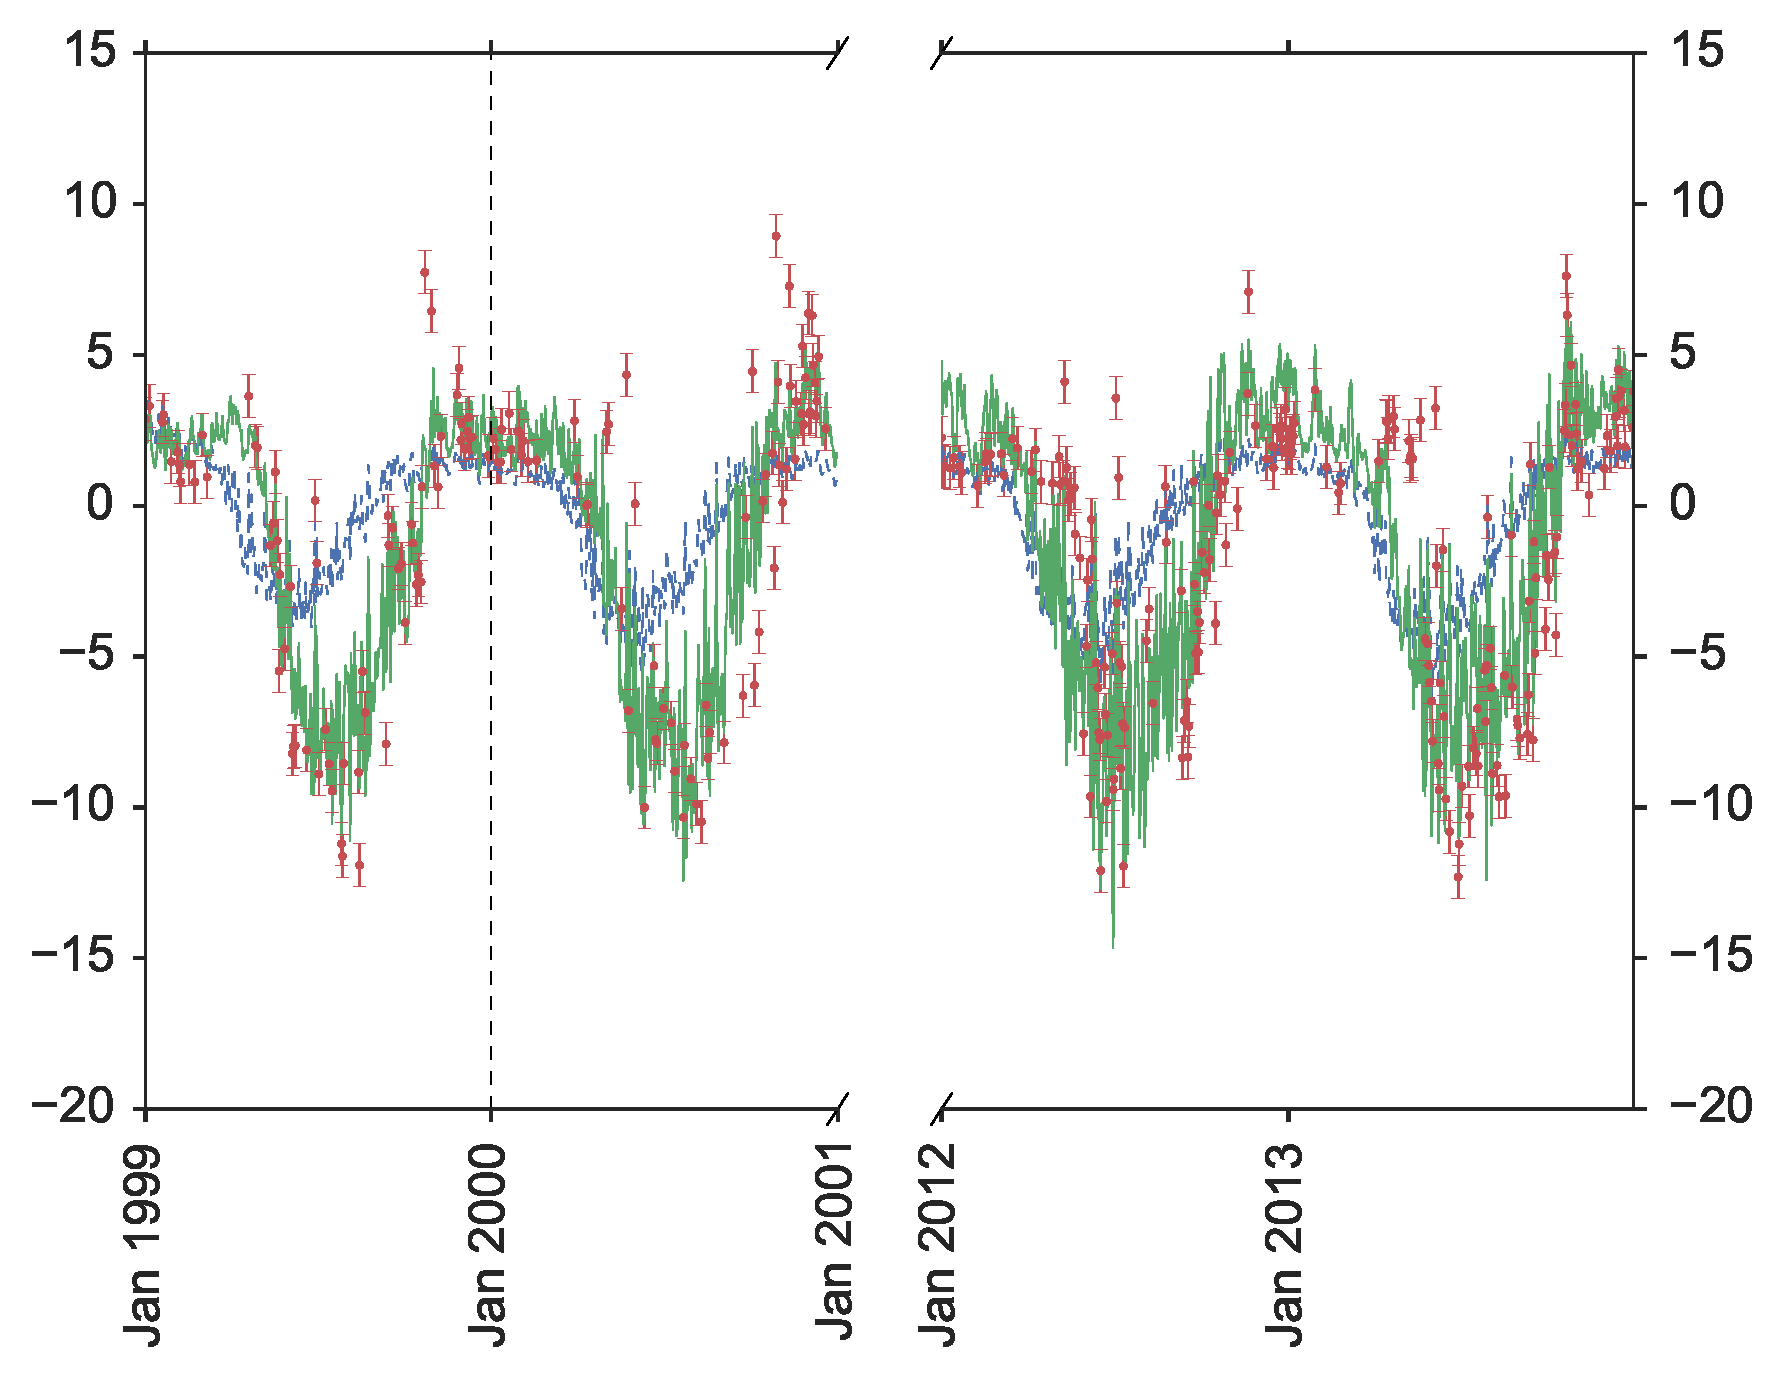
\includegraphics[width=\textwidth]{Bbroke4dvarcvt.eps}
        \caption{Experiment B}
        \label{fig:4dvaredcBR}
    \end{subfigure}
    \begin{subfigure}[b]{0.49\textwidth}
        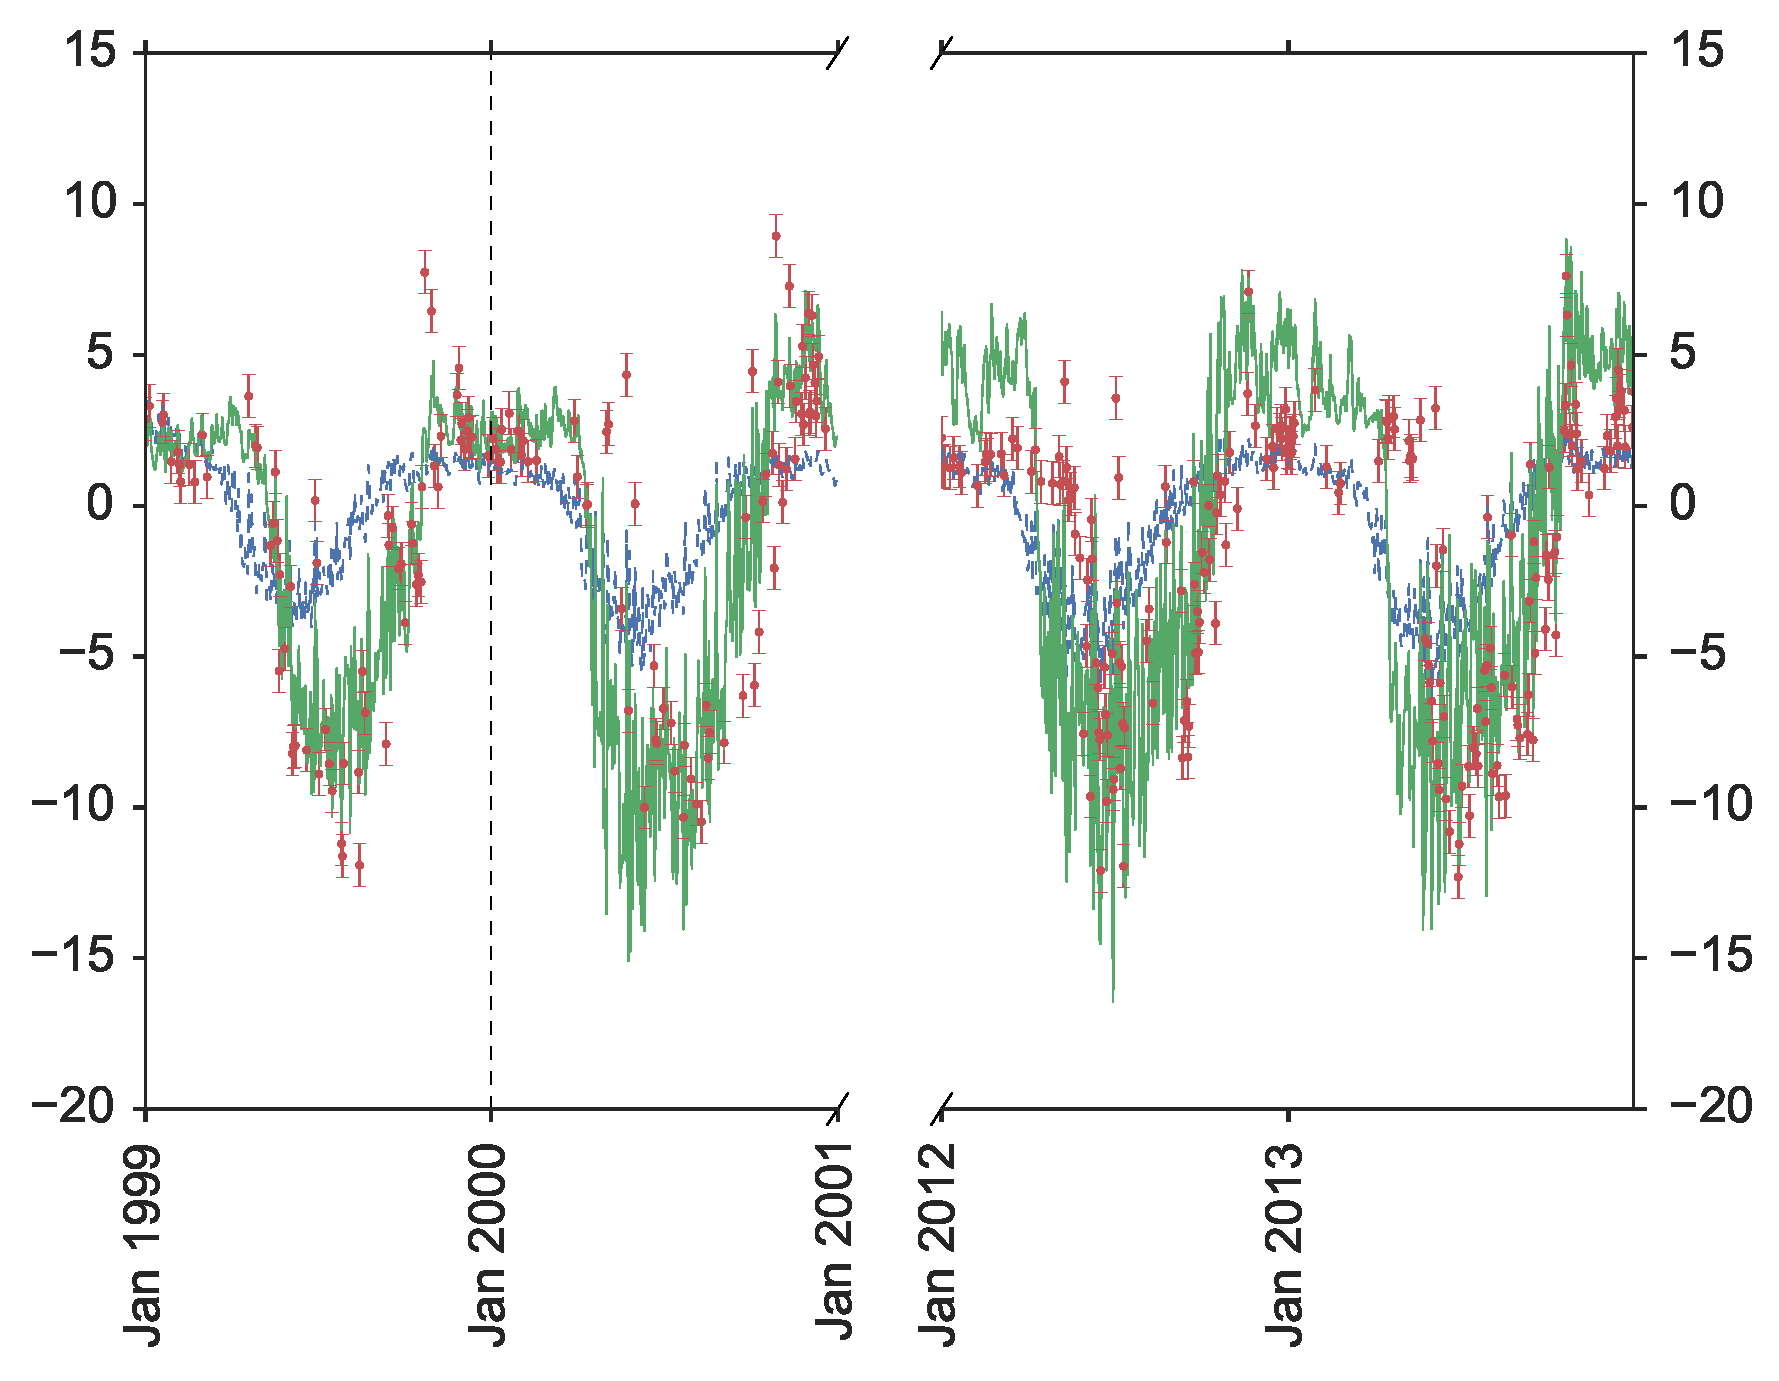
\includegraphics[width=\textwidth]{Cbroke4dvarcvt.eps}
        \caption{Experiment C}
        \label{fig:4dvarBcorR}
    \end{subfigure}
    \begin{subfigure}[b]{0.49\textwidth}
        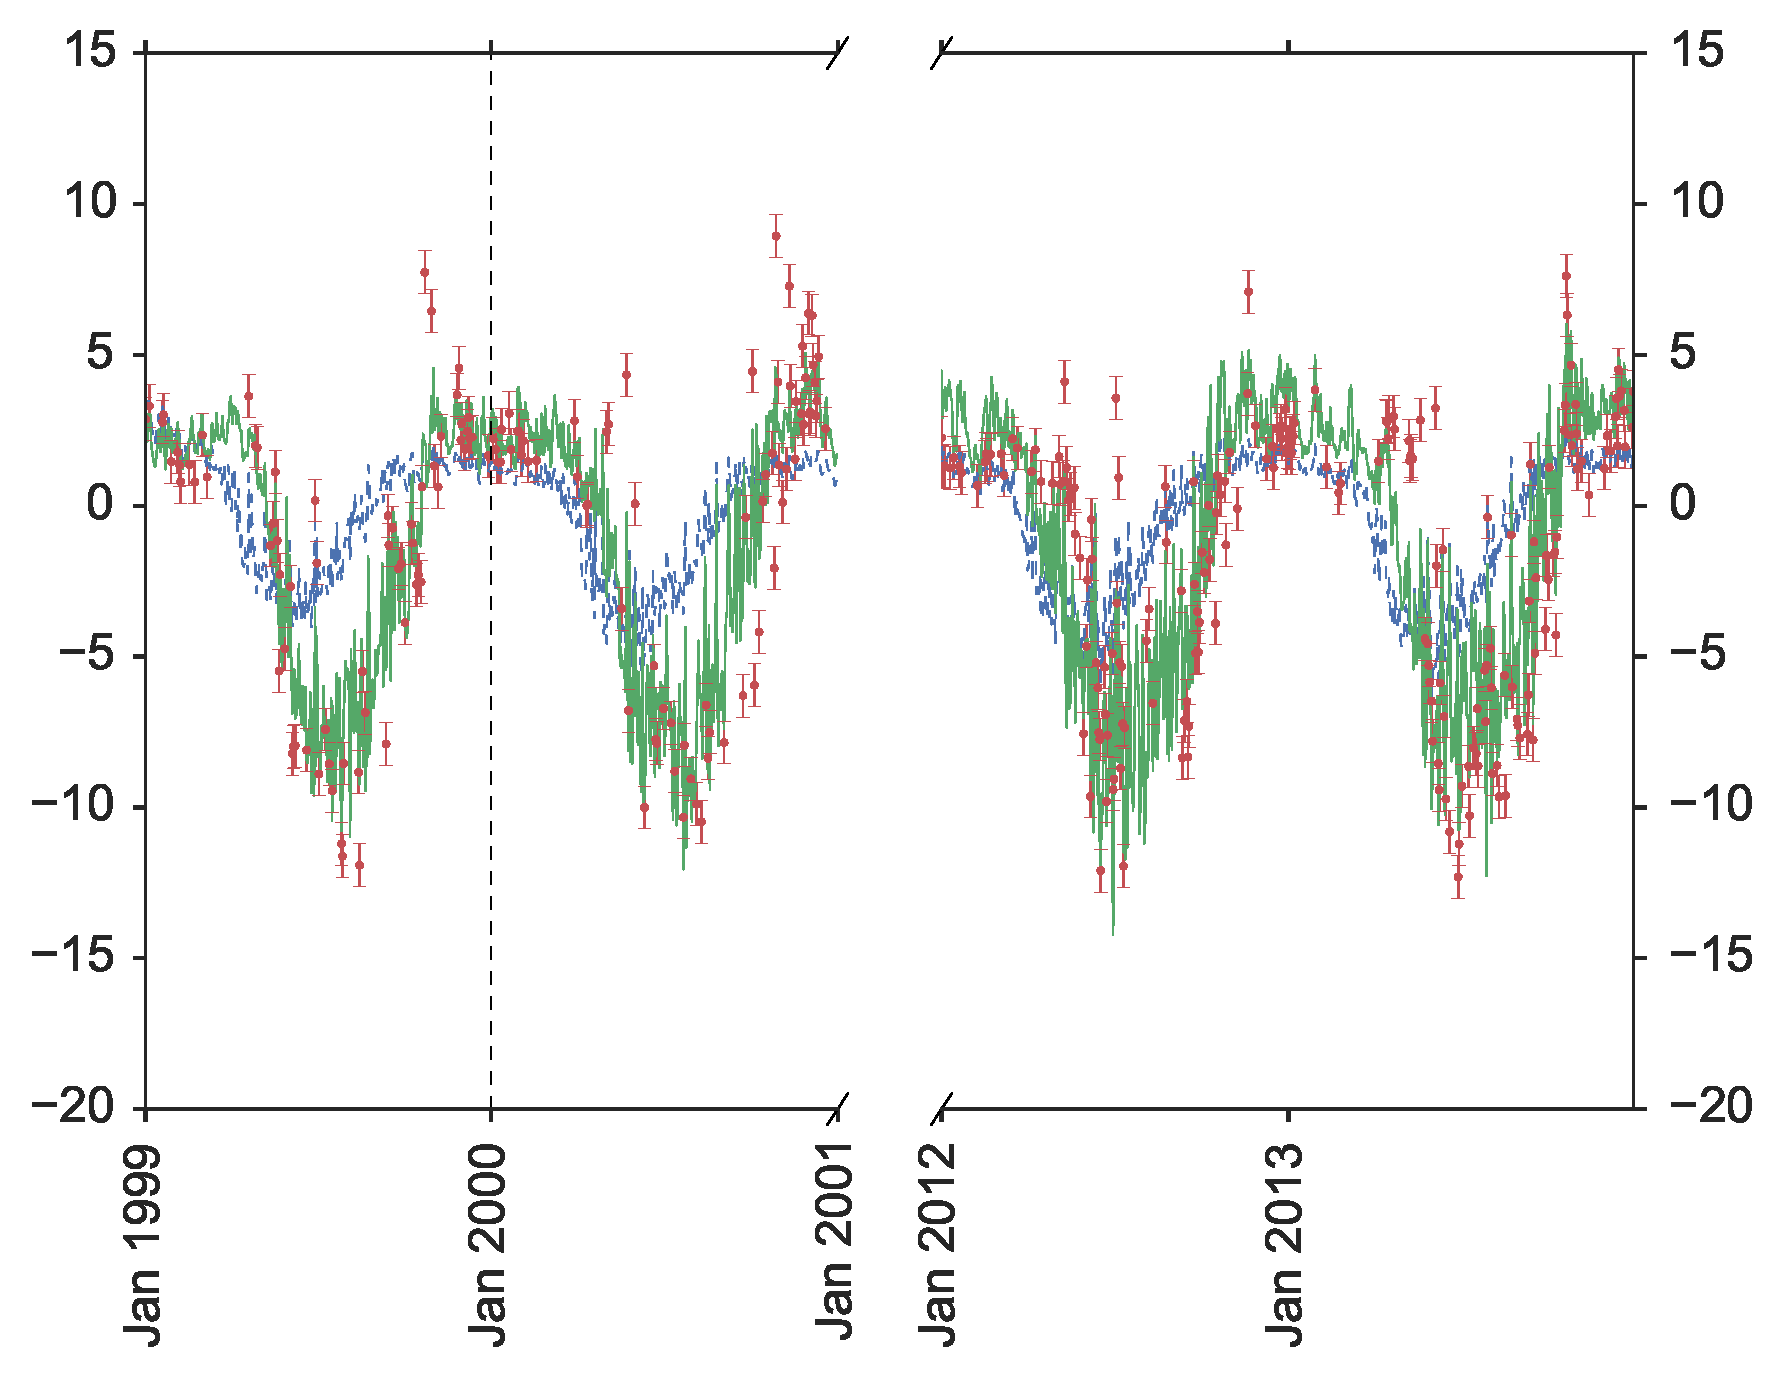
\includegraphics[width=\textwidth]{Dbroke4dvarcvt.eps}
        \caption{Experiment D}
        \label{fig:4dvaredcBcorR}
    \end{subfigure}
    \caption{Broken CVT: One year assimilation and fourteen year forecast of Alice Holt NEE with DALEC2, blue dotted line: background model trajectory, green line: analysis and forecast after assimilation, red dots: observations from Alice Holt flux site with error bars.}\label{fig:4dvar}
\end{figure}

\begin{figure}[ht]
    \centering
    \begin{subfigure}[b]{0.49\textwidth}
        \includegraphics[width=\textwidth]{td.eps}
        \caption{Taylor diagram}
        \label{fig:forecastscatBR}
    \end{subfigure}
    \begin{subfigure}[b]{0.49\textwidth}
        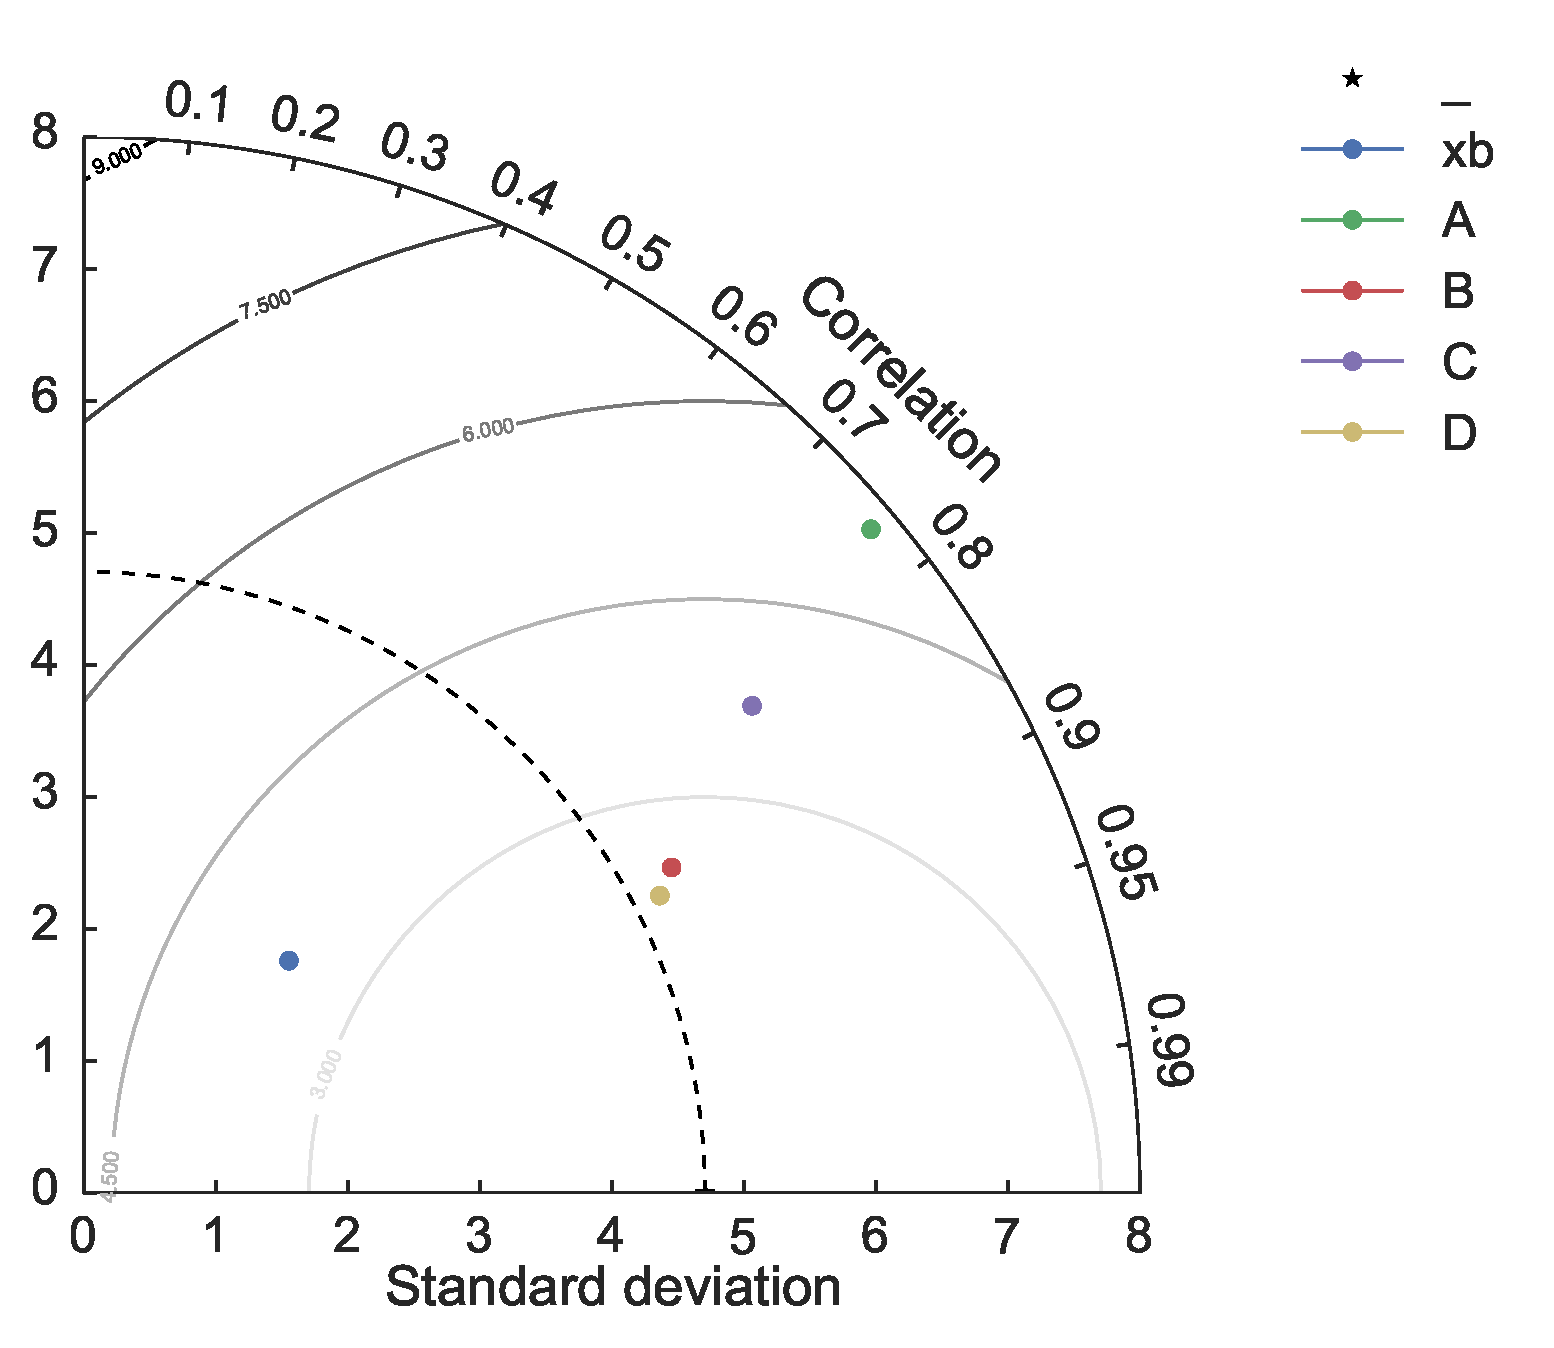
\includegraphics[width=\textwidth]{td_cvt.eps}
        \caption{CVT Taylor diagram}
        \label{fig:forecastscatedcBR}
    \end{subfigure}
    \caption{Taylor diagrams displaying statistical comparison of the four experiment and background forecast (2000-2014) results with observations of NEE $( \text{gCm}^{-2})$.}
    \label{fig:taylordiag}
\end{figure}

\begin{figure}
    \centering
    \begin{subfigure}[b]{0.49\textwidth}
        \includegraphics[width=\textwidth]{Afscatcvt.png}
        \caption{Experiment A}
        \label{fig:forecastscatBR}
    \end{subfigure}
    \begin{subfigure}[b]{0.49\textwidth}
        \includegraphics[width=\textwidth]{Bfscatcvt.png}
        \caption{Experiment B}
        \label{fig:forecastscatedcBR}
    \end{subfigure}
    \begin{subfigure}[b]{0.49\textwidth}
        \includegraphics[width=\textwidth]{Cfscatcvt.png}
        \caption{Experiment C}
        \label{fig:forecastscatBcorR}
    \end{subfigure}
    \begin{subfigure}[b]{0.49\textwidth}
        \includegraphics[width=\textwidth]{Dfscatcvt.png}
        \caption{Experiment D}
        \label{fig:forecastscatedcBcorR}
    \end{subfigure}
    \caption{CVT Forecast scatter plot of modelled NEE vs. observations for 2000-2014 (green dots). Blue line represents the 1-1 line.}\label{fig:animals}
\end{figure}

\begin{table}[ht] 
\begin{center}
	\begin{tabular}{| l | l | l | l | l |}
	\hline
	Experiment & RMSE $( \text{gCm}^{-2})$ & Bias $( \text{gCm}^{-2})$ & Correlation coefficient & \pbox{5cm}{Minimisation function \\ evaluations} \\ \hline
	Background & $3.86$ & $-1.60$ & $0.70$ & $n/a$ \\ \hline
	A & $1.36$ & $-0.02$ & $0.96$ & $431$ \\ \hline
	B & $1.40$ & $-0.03$ & $0.95$ & $298$  \\ \hline
	C & $1.37$ & $-0.09$ & $0.96$ & $259$ \\ \hline
	D & $1.41$ & $-0.08$ & $0.95$ & $279$ \\ 
	\hline
	\end{tabular}
	\caption{CVT Analysis (1999-2000) results for experiments and background when judged against observed NEE.}
	\label{table:exps_tab}
\end{center} 
\end{table}

\begin{table}[ht] 
\begin{center}
	\begin{tabular}{| l | l | l | l | l |}
	\hline
	Experiment & RMSE $( \text{gCm}^{-2})$ & Bias $( \text{gCm}^{-2})$ &  Correlation coefficient & \pbox{6cm}{Minimisation function \\ evaluations} \\ \hline
	Background & $3.86$ & $-1.36$ & $0.66$ & $n/a$ \\ \hline
	A & $5.22$ & $-0.61$ & $0.76$ & $571$ \\ \hline
	B & $2.49$ & $-0.26$ & $0.87$ & $353$  \\ \hline
	C & $3.76$ & $-0.63$ & $0.81$ & $444$ \\ \hline
	D & $2.31$ & $-0.39$ & $0.89$ & $316$ \\ 
	\hline
	\end{tabular}
	\caption{CVT Forecast (2000-2014) results for experiments and background when judged against observed NEE.}
	\label{table:exps_tab}
\end{center} 
\end{table}


\begin{figure}[ht]
    \centering
    \includegraphics[width=0.8\textwidth]{cvtinc.eps}
    \caption{CVT: Analysis increment for the four experiments.}
    \label{fig:testgradcostone}
\end{figure}


\end{document}